\documentclass[12pt]{article}
\usepackage{graphicx}
\usepackage{enumitem}
\usepackage{amsmath}
\usepackage{gvv-book}
\usepackage{gvv}

\title{\textbf{1.4.21}}
\author{\textbf{ee25btech11006 - ADUDOTLA SRIVIDYA}}
\date {september 11, 2025}

\begin{document}

\maketitle

\section*{Question}
Find the coordinates of the point which divides the line segment joining the points $(1,-2,3)$ and $(3,4,-5)$ in the ratio  

(a) $2:3$ internally,  

(b) $2:3$ externally.  

\subsection*{Solution}

Let the two points be  
\begin{align}
\vec{A} = \myvec{1 \\ -2 \\ 3}, \quad \vec{B} = \myvec{3 \\ 4 \\ -5}
\end{align}

\textbf{(a) Internal Division:}  
If \vec{P} divides \vec{AB} in the ratio $k:1$ internally, then
\begin{align}
\vec{P} = \frac{kB+A}{k+1}
\end{align}
Substituting $k=\dfrac{2}{3}$ :
\begin{align}
\vec{P} = \frac{\dfrac{2}{3}\myvec{3 \\ 4 \\ -5} + \myvec{1 \\ -2 \\ 3}}{\dfrac{5}{3}}
\end{align}
\begin{align}
\vec{P} = \frac{\myvec{2 \\ \dfrac{8}{3} \\ \dfrac{-10}{3}} + \myvec{1 \\ -2 \\ 3}}{\dfrac{5}{3}}
= \frac{\myvec{3 \\ \dfrac{2}{3} \\ \dfrac{-1}{3}}}{\dfrac{5}{3}}
= \myvec{\tfrac{9}{5} \\ \tfrac{2}{5} \\ \tfrac{-1}{5}}
\end{align}

\textbf{(b) External Division:}  
If \vec{Q} divides \vec{AB} in the ratio $k:1$ externally, then
\begin{align}
\vec{Q} = \frac{kB-A}{k-1}
\end{align}
Substituting $k=\dfrac{2}{3}$:
\begin{align}
\vec{Q} = \frac{\dfrac{2}{3}\myvec{3 \\ 4 \\ -5} - \myvec{1 \\ -2 \\ 3}}{\dfrac{5}{3}}
\end{align}
\begin{align}
\vec{Q} = \frac{\myvec{2 \\ \dfrac{8}{3} \\ \dfrac{-10}{3}} - \myvec{1 \\ -2 \\ 3}}{\dfrac{-1}{3}}
= \frac{\myvec{1 \\ \dfrac{14}{3} \\ \dfrac{-19}{3}}}{\dfrac{-1}{3}}
= \myvec{-3 \\ -14 \\ 19}
\end{align}

\begin{align}
\boxed{\text{Internal point: } \myvec{1.8 \\ 0.40 \\ -0.20}}, \quad
\boxed{\text{External point: } \myvec{-3 \\ -14 \\ 19}}
\end{align}
\begin{figure}[H]
\centering
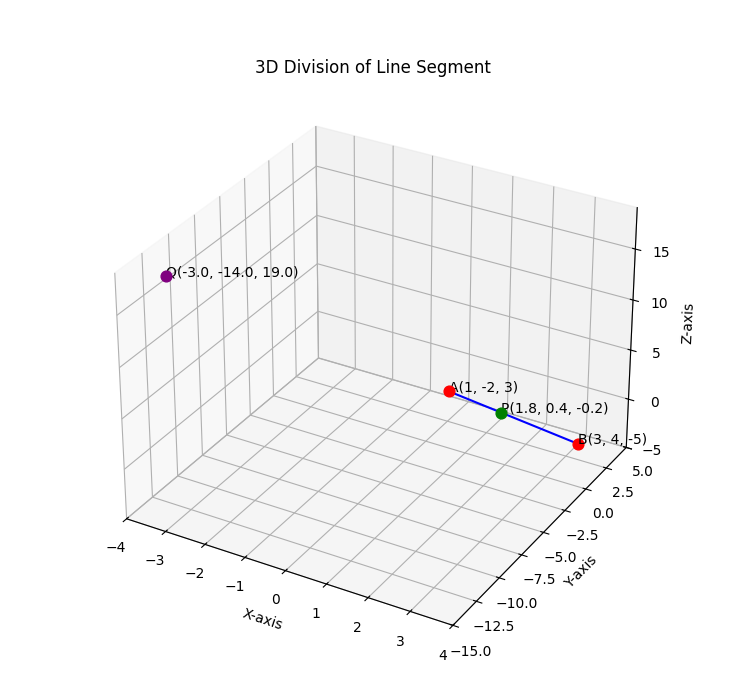
\includegraphics[width = 1.1\columnwidth]{figs/fig1.png}
\caption{3D Plot}
\label{fig1:plot}
\end{figure}
\end{document}